\documentclass[11pt]{amsart}

\usepackage[T1]{fontenc}
\usepackage{lmodern}
\usepackage{amssymb,amsmath}
\usepackage{graphicx}
\usepackage{enumitem}
\usepackage[dvipsnames]{xcolor}
\usepackage[margin=1.15in]{geometry}
\usepackage{microtype}
\usepackage{xurl}
\usepackage[colorlinks=true,linkcolor=blue!50!black,citecolor=blue!50!black,urlcolor=blue!50!black]{hyperref}
\emergencystretch=3em

\newtheorem{theorem}{Theorem}[section]
\newtheorem{proposition}[theorem]{Proposition}
\newtheorem{lemma}[theorem]{Lemma}
\newtheorem{corollary}[theorem]{Corollary}
\newtheorem{introthm}{Theorem}
\newtheorem{introcor}[introthm]{Corollary}
\theoremstyle{definition}
\newtheorem{definition}[theorem]{Definition}
\theoremstyle{remark}
\newtheorem{remark}[theorem]{Remark}
\numberwithin{equation}{section}

\newcommand{\N}{\mathbb{N}}
\newcommand{\Z}{\mathbb{Z}}
\newcommand{\Q}{\mathbb{Q}}
\newcommand{\R}{\mathbb{R}}
\newcommand{\C}{\mathbb{C}}
\newcommand{\A}{\mathbb{A}}
\newcommand{\cU}{\mathcal{U}}
\newcommand{\ind}[1]{[\,#1\,]}
\DeclareMathOperator{\lcm}{lcm}
\DeclareMathOperator{\lc}{lc}
\DeclareMathOperator{\ord}{ord}
\DeclareMathOperator{\wt}{wt}
\DeclareMathOperator{\length}{length}
\DeclareMathOperator{\sgn}{sgn}
\providecommand{\doi}[1]{\href{https://doi.org/#1}{doi:\nolinkurl{#1}}}
\hypersetup{pdftitle={Degrees of Prolongation Varieties of Monomial Planar Systems},pdfauthor={Deep Bhattacharjee}}

\begin{document}

\title{Degrees of Prolongation Varieties of Monomial Planar Systems}

\author{Deep Bhattacharjee}
\address{Formerly, Electro-Gravitational Space Propulsion Laboratory (EGSPL),\newline Bhubaneswar, Odisha 751030, India\newline
Formerly, University of Calcutta (Heramba Chandra College),\newline 23/49 Gariahat Road, Golpark, Kolkata 700029, West Bengal, India}
\email{d.bhattacharjee@erl-forschung.de}
\email{itsdeep@live.com}
\email{egspl@proton.me}
\urladdr{https://orcid.org/0000-0003-0466-750X}
\urladdr{https://github.com/creelie}
\thanks{Corresponding author: Deep Bhattacharjee, \href{mailto:d.bhattacharjee@erl-forschung.de}{d.bhattacharjee@erl-forschung.de}; ORCID \href{https://orcid.org/0000-0003-0466-750X}{\mbox{0000-0003-0466-750X}}. For the code and data: \href{mailto:egspl@proton.me}{egspl@proton.me} (GitHub: creelie).}

\subjclass[2020]{12H05, 14N10, 14H50, 13D40, 26C10}
\keywords{prolongation variety, geometric degree, differential algebra, weighted B\'ezout theorem, interlacing zeros}

\begin{abstract}
For the differential system $x_1'=x_2^p$, $x_2'=x_1^q$ with $p,q\ge2$ we compute the degree of every prolongation variety. It is a quadratic quasi-polynomial in the order of prolongation, with period $\lcm(p+1,q+1)$. This proves the two formulas proposed by Pogudin, gives the quasi-polynomial he asked for when $(p,q)=(2,3)$, and proves Puddu's conjecture.
\end{abstract}

\maketitle

\section{Introduction}\label{sec:intro}

Let $K$ be an algebraically closed field of characteristic zero, regarded as a differential field with the zero derivation, and let $f_1,\dots,f_\ell$ be differential polynomials in $x_1,\dots,x_n$. The $m$-th prolongation of the system $f_1=\dots=f_\ell=0$ is the affine variety
\[
X_m=V\bigl(f_i^{(h)}:1\le i\le\ell,\ 0\le h\le m\bigr),
\]
cut out by the equations and their first $m$ derivatives in the finitely many jet coordinates that occur \cite{Ritt,Pog25}. Prolongations are the finite-dimensional shadows of the differential system, and their dimension, components and degree govern the cost of methods that truncate a differential problem at a finite order. Pogudin \cite[Section~2]{Pog25} singled out the case of a polynomial dynamical system $x'=P(x)$. Here $X_m$ is irreducible of dimension $n$ for every $m$, so the only invariant left to determine is its degree.\footnote{The degree of an irreducible affine variety of dimension $d$ is the number of points in which a generic affine linear subspace of codimension $d$ meets it \cite[Lecture~18]{Har92}. For $X_m$ it depends on the embedding by jet coordinates, not only on the abstract variety.}

Already for $n=2$ the answer is not obvious. For the systems
\[
F_1:\ x_1'=x_2^2,\ x_2'=x_1^2,\qquad F_2:\ x_1'=x_2^3,\ x_2'=x_1^3,
\]
Pogudin computed $\deg X_m$ for $m\le10$ and proposed
\begin{equation}\label{eq:pogudin}
\deg X_m(F_1)=(m+2)^2-2\,\ind{m\equiv1\ (3)},\qquad
\deg X_m(F_2)=(2m+3)^2-8\,\ind{m\equiv1,2\ (4)},
\end{equation}
asking for a proof (Question~6 of \cite{Pog25}). He also asked whether $\deg X_m$ is always a quasi-polynomial in $m$ and how it depends on the system (Question~7), and, for
\[
F_3:\ x_1'=x_2^2,\ x_2'=x_1^3,
\]
listed the values $6,11,26,46,66,91,121,156,196$ and asked what the quasi-polynomial would be. Upper bounds for $F_1$ were found by Jeronimo and by Falkensteiner and Sendra.\footnote{Both are reported in \cite[Section~2]{Pog25} as personal communications.} Lanciano \cite{Lan26} proved $\deg X_1\le(\deg X_0)^2$ for systems with a smooth irreducible zero set and a prime defining ideal, which gives $16$ for $F_1$ against the true value $7$. Puddu \cite{Pud26} proved the first formula in \eqref{eq:pogudin} with algebraic Thomas decompositions and an interlacing argument, and conjectured for $x_1'=x_2^n$, $x_2'=x_1^n$ the formula $\deg X_m=((n-1)m+n)^2-2(n-1)r(n-r)$, where $m\equiv r\pmod{n+1}$ \cite[Conjecture~4.1]{Pud26}.

We settle these questions for the whole two-parameter family
\[
F_{p,q}:\qquad x_1'=x_2^{\,p},\qquad x_2'=x_1^{\,q}\qquad(p,q\ge2).
\]

\begin{introthm}\label{thm:main}
Let $p,q\ge2$, put $c=pq-1$, and for $m\ge0$ let $r\in\{0,\dots,p\}$ and $s\in\{0,\dots,q\}$ be the residues of $m$ modulo $p+1$ and $q+1$. Then
\[
\deg X_m(F_{p,q})=\frac{\bigl(p(q+1)+mc\bigr)\bigl(q(p+1)+mc\bigr)}{(p+1)(q+1)}-c\left(\frac{r(p-r)}{p+1}+\frac{s(q-s)}{q+1}\right).
\]
\end{introthm}

The first term is a weighted B\'ezout number and the bracket records two points at infinity, one on each coordinate axis, at which the generic linear section of $X_m$ escapes to infinity; Figure~\ref{fig:defect} shows the bracket for $(p,q)=(3,4)$. For $m=0$ the formula gives $pq$, the degree of the graph of $(x_2^p,x_1^q)$.

\begin{figure}[ht]
\centering
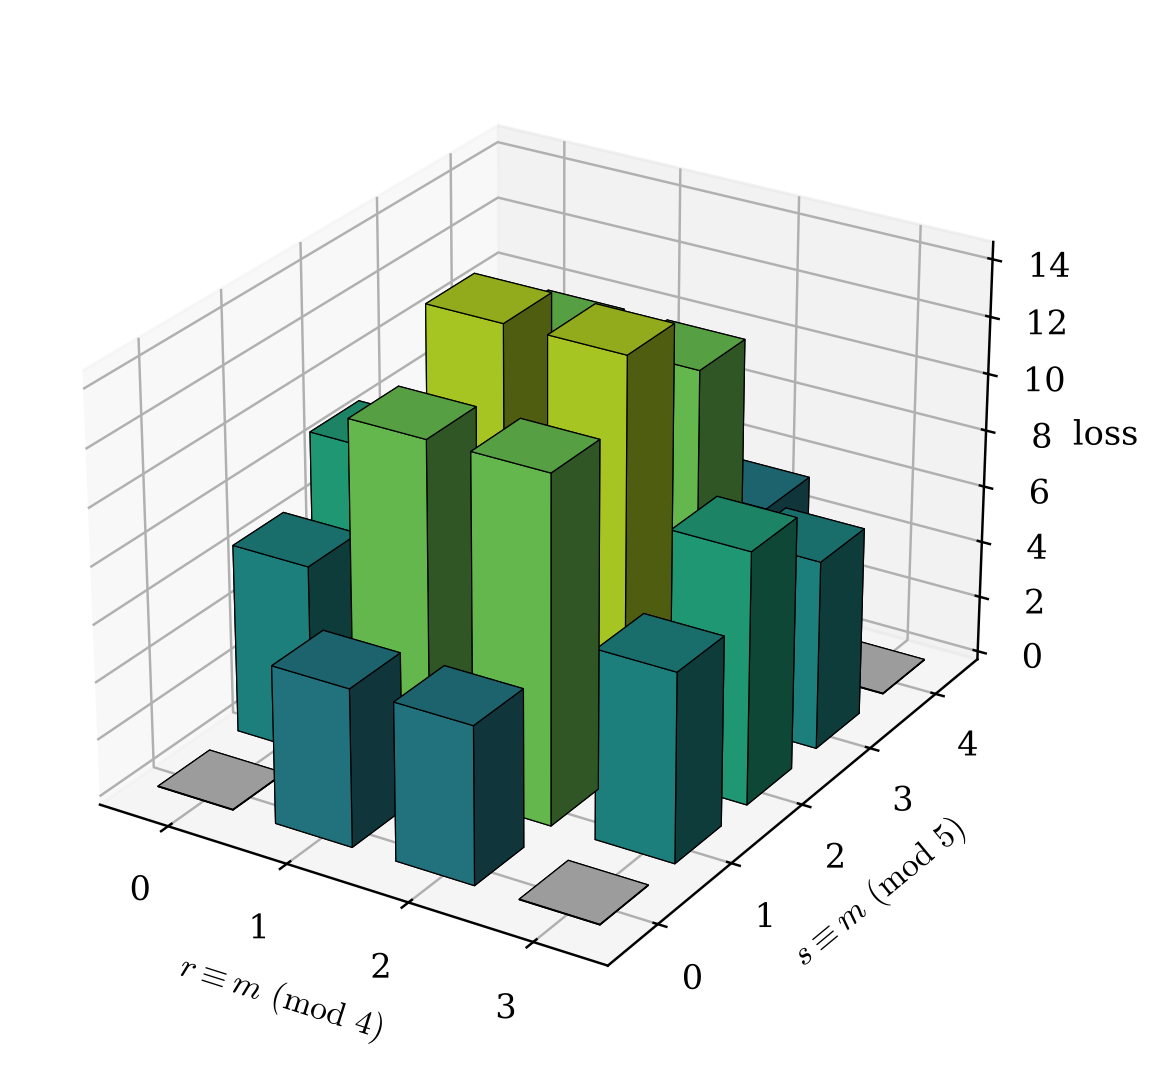
\includegraphics[width=0.82\textwidth]{fig_defect.png}
\caption{The loss $c\bigl(r(p-r)/(p+1)+s(q-s)/(q+1)\bigr)$ in Theorem~\ref{thm:main} for $(p,q)=(3,4)$, $c=11$, over the residues $r$ of $m$ modulo $4$ and $s$ modulo $5$. The bars on the edges $r\in\{0,p\}$ and $s\in\{0,q\}$ come from one point at infinity only; the loss is zero exactly when $r\in\{0,p\}$ and $s\in\{0,q\}$.}
\label{fig:defect}
\end{figure}

\begin{introcor}\label{cor:pogudin}
\begin{enumerate}[label=\textup{(\roman*)},leftmargin=*]
\item Both formulas \eqref{eq:pogudin} hold for every $m\ge0$. More generally, for $p=q=n\ge2$ one has $\deg X_m=((n-1)m+n)^2-2(n-1)r(n-r)$ with $r\equiv m\pmod{n+1}$, which is Puddu's conjecture.
\item For $F_3$, with $r\equiv m\pmod3$ and $s\equiv m\pmod4$,
\[
\deg X_m(F_3)=\frac{(5m+8)(5m+9)-20\,r(2-r)-15\,s(3-s)}{12},
\]
which gives $6,11,26,46,66,91,121,156,196,236,281,\dots$ for $m=0,1,2,\dots$.
\item For every $p,q\ge2$ the sequence $\deg X_m(F_{p,q})$ is a quasi-polynomial of degree two in $m$, with leading coefficient $(pq-1)^2/\bigl((p+1)(q+1)\bigr)$ and periodic part of period $\lcm(p+1,q+1)$.
\end{enumerate}
\end{introcor}

The prolongation $X_m$ is the graph of the map $(a,b)\mapsto(A_l(a,b),B_l(a,b))_{1\le l\le m+1}$, where $A_l$ and $B_l$ are the iterates of $a$ and $b$ under the derivation $D=b^p\partial_a+a^q\partial_b$ (Lemma~\ref{lem:graph}). The second ingredient of the proof, which is of independent interest, describes their common factor; for $p=q$ it is the gcd statement of \cite[Conjecture~4.1]{Pud26}.

\begin{introthm}\label{thm:gcd}
Let $p,q\ge1$ and $l\ge1$, and let $r\in\{0,\dots,p\}$, $s\in\{0,\dots,q\}$ be the residues of $l-1$ modulo $p+1$ and $q+1$. Every common zero of $A_l$ and $B_l$ in $K^2$ lies on the coordinate axes, and
\[
\gcd(A_l,B_l)=a^{(q-s)\ind{s\ge1}}\,b^{(p-r)\ind{r\ge1}}.
\]
\end{introthm}

\subsection*{Method}
Theorem~\ref{thm:main} is proved in three steps. First, $D$ is homogeneous for the weights $\wt a=(p+1)/g$, $\wt b=(q+1)/g$ with $g=\gcd(p+1,q+1)$, and a generic linear section of $X_m$ is the zero set of $A_{m+1}+U$ and $B_{m+1}+V$ with $U,V$ of lower weight. In the weighted projective plane the two curves meet in a number of points given by their Hilbert series, and the affine count is that number minus the intersection multiplicities at infinity (Section~\ref{sec:bezout}). Second, Theorem~\ref{thm:gcd} shows that the only possible points at infinity are the two axis points. We prove it by transporting $A_l$ and $B_l$ to a real arc of the curve $u^{p+1}+v^{q+1}=1$, where they become successive derivatives along a flow, and by showing that their zeros on the arc interlace at every order (Section~\ref{sec:interlacing}). Third, at each axis point both curves have a Newton polygon with a single edge, which gives the multiplicities $c\,r(p-r)/g$ and $c\,s(q-s)/g$ (Section~\ref{sec:local}).

For $p=q$ the jets are homogeneous, the two points at infinity are exchanged by the symmetry $a\leftrightarrow b$, and the real arc is the curve of the squigonometric functions of van Lith \cite{vL25}.\footnote{For $p=q=n$ the flow of Section~\ref{sec:interlacing}, rescaled by $n+1$, is $u'=v^n$, $v'=-u^n$ on $u^{n+1}+v^{n+1}=1$; for general $p,q$ the arc is of the kind studied for generalised trigonometric functions \cite{EGL12}.} Puddu indicated in \cite[Section~4]{Pud26} that the multiplicity at each axis point should be $(n-1)r(n-r)$, and a proof outline for $p=q$ along these lines was posted on 5 November 2026 in a public issue of a formalisation project.\footnote{Issue \#26996 of the repository \url{https://github.com/the-omega-institute/trureturing}, which records the outline and no formal proof.} When $p\neq q$ the jets are only weighted homogeneous, the two axis points carry different multiplicities, and the relation between $A_l$ and $B_l$ on the arc is no longer a reflection; Sections~\ref{sec:bezout}--\ref{sec:local} treat the general case directly and contain the case $p=q$.

Exact formulas that pin down, for a whole family, a count first known from computation are also the subject of the author's earlier work on Lehmer's totient problem \cite{BhaLehmer}, on class groups of small exponent \cite{BhaClass} and on Tate--Shafarevich groups \cite{BhaBSD}.

\subsection*{Organisation}
Section~\ref{sec:jets} sets up the jets and their weights. Section~\ref{sec:interlacing} proves Theorem~\ref{thm:gcd}. Section~\ref{sec:bezout} reduces the degree to two local intersection numbers, Section~\ref{sec:local} computes them, and Section~\ref{sec:proof} completes the proofs. No step relies on a computer; the values in Corollary~\ref{cor:pogudin}(ii) agree with those listed in \cite{Pog25}.

\section{The jets and their weights}\label{sec:jets}

Throughout, $p,q\ge1$ are integers, $N=p+1$, $M=q+1$, and for an integer $t$ and a modulus $k$ we write $t\bmod k$ for the residue in $\{0,\dots,k-1\}$. The bracket $\ind{P}$ is $1$ if $P$ holds and $0$ otherwise. On $K[a,b]$ let
\[
D=b^p\frac{\partial}{\partial a}+a^q\frac{\partial}{\partial b},\qquad A_l=D^l(a),\qquad B_l=D^l(b)\qquad(l\ge0).
\]

\begin{lemma}\label{lem:graph}
Let $f_1=x_1'-x_2^p$ and $f_2=x_2'-x_1^q$. For every $m\ge0$ the ideal generated by $f_i^{(h)}$, $i=1,2$, $0\le h\le m$, equals the ideal generated by $x_1^{(l)}-A_l(x_1,x_2)$ and $x_2^{(l)}-B_l(x_1,x_2)$, $1\le l\le m+1$. Hence $X_m\subset\A^{2(m+2)}$ is the graph of $(a,b)\mapsto(A_l(a,b),B_l(a,b))_{1\le l\le m+1}$, and $X_m\cong\A^2$.
\end{lemma}

\begin{proof}
Write $I_h$ for the ideal generated by $f_i^{(k)}$, $k\le h$, and $J_h$ for the ideal generated by $x_1^{(l)}-A_l$ and $x_2^{(l)}-B_l$, $1\le l\le h+1$; thus $J_0=I_0=(f_1,f_2)$. For $g\in K[x_1,x_2]$ the chain rule gives $g'=g_{x_1}x_1'+g_{x_2}x_2'\equiv(Dg)(x_1,x_2)$ modulo $J_0$. Applied to the generators of $J_{h-1}$, this shows $J_{h-1}'\subseteq J_h$, since $(x_1^{(l)}-A_l)'\equiv x_1^{(l+1)}-A_{l+1}$ modulo $J_0$, and similarly for $x_2$. Applied repeatedly to $g$, it gives $g^{(h)}\equiv(D^hg)(x_1,x_2)$ modulo $J_{h-1}$. With $g=x_2^p$ and $g=x_1^q$, and since $A_{h+1}=D^h(b^p)$ and $B_{h+1}=D^h(a^q)$, we get
\[
f_1^{(h)}\equiv x_1^{(h+1)}-A_{h+1},\qquad f_2^{(h)}\equiv x_2^{(h+1)}-B_{h+1}\qquad\text{modulo }J_{h-1}.
\]
Hence $I_h\subseteq J_h$, and by induction on $h$ also $J_h\subseteq I_h+J_{h-1}\subseteq I_h$.
\end{proof}

Let $V_m\subset K[a,b]$ be the span of $1,A_0,B_0,\dots,A_m,B_m$.

\begin{lemma}\label{lem:degcount}
There is a dense open set $\Omega\subset V_m\times V_m$ such that for $(U,V)\in\Omega$ the polynomials $F=A_{m+1}+U$, $G=B_{m+1}+V$ satisfy
\[
\deg X_m=\dim_K K[a,b]/(F,G),
\]
and every common zero of $F$ and $G$ is a simple one.
\end{lemma}

\begin{proof}
An affine subspace of codimension two is the zero set of two affine linear forms $\lambda_i=c_{i}+\sum_{l\le m+1}(u_{il}x_1^{(l)}+v_{il}x_2^{(l)})$. By Lemma~\ref{lem:graph}, its intersection with $X_m$ is identified with the zero set in $K^2$ of $\lambda_i(A_\bullet,B_\bullet)$. If the $2\times2$ matrix $(u_{i,m+1},v_{i,m+1})$ is invertible, which is an open condition, a linear change of the two forms, which does not change their zero set, brings them to $F=A_{m+1}+U$ and $G=B_{m+1}+V$ with $U,V\in V_m$, and every pair $(U,V)$ arises. For a generic subspace the intersection consists of $\deg X_m$ points, at each of which it is transversal \cite[Lectures~17 and~18]{Har92}. These conditions depend only on the zero set and define a dense open set of subspaces, so the pairs $(U,V)$ for which they hold form a dense open set $\Omega$. Since $X_m\cong\A^2$ through $(a,b)$, transversality at a point means that $dF$ and $dG$ are independent there, that is, the local ring of $K[a,b]/(F,G)$ at the point is $K$.
\end{proof}

\subsection{Weights}
Let $g=\gcd(N,M)$ and
\[
\alpha=\frac{N}{g},\qquad \beta=\frac{M}{g},\qquad \delta=\frac{pq-1}{g},\qquad L=\frac{NM}{g}=N\beta=M\alpha .
\]
These are integers ($pq-1=(p+1)(q+1)-N-M$), and $p\beta=\alpha+\delta$, $q\alpha=\beta+\delta$. Give $a$ weight $\alpha$ and $b$ weight $\beta$. Then $D$ raises weights by $\delta$, so $A_l$ and $B_l$ are weighted homogeneous of weights
\[
W_A(l)=\alpha+l\delta,\qquad W_B(l)=\beta+l\delta .
\]
For $p,q\ge2$ we have
\begin{equation}\label{eq:deltabig}
\delta-|\alpha-\beta|=\frac{pq-1-|p-q|}{g}=\frac{(\min(p,q)-1)(\max(p,q)+1)}{g}>0 .
\end{equation}

On a monomial, $D(a^ib^j)=i\,a^{i-1}b^{j+p}+j\,a^{i+q}b^{j-1}$. Both terms lower $i$ by one modulo $M$ and $j$ by one modulo $N$, and both have nonnegative coefficients. Put
\[
\rho_l=(-l)\bmod N,\quad \sigma_l=(1-l)\bmod M,\quad \rho'_l=(1-l)\bmod N,\quad \sigma'_l=(-l)\bmod M .
\]

\begin{lemma}\label{lem:extreme}
The coefficients of $A_l$ and $B_l$ are nonnegative integers. Every monomial $a^ib^j$ of $A_l$ has $j\equiv\rho_l\pmod N$ and $i\equiv\sigma_l\pmod M$; every monomial of $B_l$ has $j\equiv\rho'_l$ and $i\equiv\sigma'_l$. Moreover $A_l$ contains a monomial with $b$-exponent exactly $\rho_l$ and one with $a$-exponent exactly $\sigma_l$, and $B_l$ contains a monomial with $b$-exponent $\rho'_l$ and one with $a$-exponent $\sigma'_l$.
\end{lemma}

\begin{proof}
The first two statements follow by induction from $A_0=a$, $B_0=b$ and the formula for $D$. Since no cancellation occurs, the monomials of $D(h)$, for $h$ with nonnegative coefficients, are the monomials of $D(a^ib^j)$ over the monomials $a^ib^j$ of $h$. Let $a^ib^j$ be a monomial of $A_l$ with $j<N$. If $j\ge1$, then $A_{l+1}$ contains $a^{i+q}b^{j-1}$. If $j=0$ then $i\ge1$, since $A_l$ has positive weight, and $A_{l+1}$ contains $a^{i-1}b^{p}$. In both cases $A_{l+1}$ has a monomial with $b$-exponent below $N$, which by the congruence equals $\rho_{l+1}$. The base case is $A_0=a$. The other three statements are proved in the same way.
\end{proof}

By Lemma~\ref{lem:extreme} the exponents of the monomials of $A_l$ are $j=\rho_l+Nt$ and $i=\sigma_l+Ms$ with $s,t\ge0$, and weighted homogeneity gives $s+t=k_A(l)$, where
\begin{equation}\label{eq:kA}
L\,k_A(l)=\alpha+l\delta-\sigma_l\alpha-\rho_l\beta,\qquad L\,k_B(l)=\beta+l\delta-\sigma'_l\alpha-\rho'_l\beta .
\end{equation}
Hence
\begin{equation}\label{eq:binaryform}
A_l=a^{\sigma_l}b^{\rho_l}\,\Pi^A_l(b^N,a^M),\qquad B_l=a^{\sigma'_l}b^{\rho'_l}\,\Pi^B_l(b^N,a^M),
\end{equation}
where $\Pi^A_l(X,Y)$ and $\Pi^B_l(X,Y)$ are binary forms of degrees $k_A(l)$ and $k_B(l)$ with nonnegative integer coefficients, and by the last part of Lemma~\ref{lem:extreme} the coefficients of $X^{k}$ and $Y^{k}$ in each of them are positive.

\begin{lemma}\label{lem:kcount}
For every $l\ge0$:
\begin{enumerate}[label=\textup{(\alph*)},leftmargin=*]
\item $k_A(l+1)=k_A(l)-1+\ind{\rho_l\ge1}+\ind{\sigma_l\ge1}$ and $k_B(l+1)=k_B(l)-1+\ind{\rho'_l\ge1}+\ind{\sigma'_l\ge1}$;
\item $k_A(l)+\ind{\rho_l=p}=k_B(l)+\ind{\sigma'_l=q}$;
\item $k_A(0)=k_B(0)=0$.
\end{enumerate}
\end{lemma}

\begin{proof}
We have $\rho_{l+1}=\rho_l-1$ if $\rho_l\ge1$ and $\rho_{l+1}=p$ if $\rho_l=0$, and similarly for $\sigma$. By \eqref{eq:kA}, $L(k_A(l+1)-k_A(l))=\delta-(\sigma_{l+1}-\sigma_l)\alpha-(\rho_{l+1}-\rho_l)\beta$. If $\rho_l,\sigma_l\ge1$ this is $\delta+\alpha+\beta=L$. If $\sigma_l=0<\rho_l$ it is $\delta-q\alpha+\beta=0$; if $\rho_l=0<\sigma_l$ it is $\delta+\alpha-p\beta=0$; if both vanish it is $\delta-q\alpha-p\beta=-L$. This is (a) for $A$, and $B$ is the same. For (b), note $\rho'_l=\rho_l+1$ if $\rho_l<p$ and $\rho'_l=0$ if $\rho_l=p$, while $\sigma_l=\sigma'_l+1$ if $\sigma'_l<q$ and $\sigma_l=0$ if $\sigma'_l=q$. Then \eqref{eq:kA} gives
\[
L\bigl(k_A(l)-k_B(l)\bigr)=\alpha-\beta-(\sigma_l-\sigma'_l)\alpha-(\rho_l-\rho'_l)\beta=L\,\ind{\sigma'_l=q}-L\,\ind{\rho_l=p}.
\]
Part (c) holds because $A_0=a$ and $B_0=b$.
\end{proof}

\section{Interlacing on a real arc}\label{sec:interlacing}

In this section $K=\C$. Since $A_l,B_l\in\Z[a,b]$, Theorem~\ref{thm:gcd} for $\C$ implies it for every algebraically closed field of characteristic zero: the greatest common divisor of two polynomials with rational coefficients does not change under field extension, and a common zero off the axes would give a common factor other than $a$ and $b$.

\subsection{The arc}
Consider the real polynomial vector field on $\R^2$
\[
\mathcal X=\frac{v^q}{N}\frac{\partial}{\partial u}-\frac{u^p}{M}\frac{\partial}{\partial v},
\]
and put $\Phi_l=\mathcal X^l(v)$ and $\Psi_l=\mathcal X^l(u)$. The function $u^N+v^M$ is a first integral, and $\mathcal X$ moves the arc
\[
\Gamma=\{(u,v)\in(0,1)^2:\ u^N+v^M=1\}
\]
from $(0,1)$ towards $(1,0)$.

\begin{lemma}\label{lem:transport}
Choose $\kappa\in\C^\times$ with $\kappa^{pq-1}=-1/(MN^p)$ and put $\mu=N\kappa^q$. The substitution $a=\kappa v$, $b=\mu u$ carries $A_l$ to $\kappa\Phi_l$ and $B_l$ to $\mu\Psi_l$. In particular $\Phi_l$ and $\Psi_l$ have the same monomials as $A_l$ and $B_l$, with $a\leftrightarrow v$ and $b\leftrightarrow u$.
\end{lemma}

\begin{proof}
Let $\tau:\C[a,b]\to\C[u,v]$ be the substitution. Then $\tau\circ D$ and $\mathcal X\circ\tau$ are derivations along $\tau$, and they agree on generators: $\tau(Da)=\mu^pu^p$ and $\mathcal X(\tau a)=-\kappa u^p/M$, which are equal because $\mu^p=N^p\kappa^{pq}=-\kappa/M$; and $\tau(Db)=\kappa^qv^q=\mu v^q/N=\mathcal X(\tau b)$. Hence $\tau(D^lh)=\mathcal X^l(\tau h)$ for all $h$, and $\tau$ maps distinct monomials to nonzero multiples of distinct monomials.
\end{proof}

By Lemma~\ref{lem:transport} and \eqref{eq:binaryform},
\[
\Phi_l=u^{\rho_l}v^{\sigma_l}\,\tilde\Pi^A_l(u^N,v^M),\qquad \Psi_l=u^{\rho'_l}v^{\sigma'_l}\,\tilde\Pi^B_l(u^N,v^M),
\]
where $\tilde\Pi^A_l(X,Y)=\kappa^{-1}\kappa^{\sigma_l}\mu^{\rho_l}\,\Pi^A_l(\mu^NX,\kappa^MY)$ and $\tilde\Pi^B_l$ is defined in the same way; these are binary forms of degrees $k_A(l)$ and $k_B(l)$, with real coefficients because $\Phi_l$ and $\Psi_l$ are real, and with nonzero coefficients of $X^k$ and $Y^k$. Parametrise $\Gamma$ by $x=u^N\in(0,1)$, so that $u=x^{1/N}$ and $v=(1-x)^{1/M}$. Then
\begin{equation}\label{eq:phipsi}
\varphi_l(x):=\Phi_l|_\Gamma=x^{\rho_l/N}(1-x)^{\sigma_l/M}F_l(x),\qquad \psi_l(x):=\Psi_l|_\Gamma=x^{\rho'_l/N}(1-x)^{\sigma'_l/M}G_l(x),
\end{equation}
where $F_l(x)=\tilde\Pi^A_l(x,1-x)$ and $G_l(x)=\tilde\Pi^B_l(x,1-x)$. Thus $\deg F_l\le k_A(l)$, $\deg G_l\le k_B(l)$, and $F_l(0)F_l(1)G_l(0)G_l(1)\neq0$.

\begin{lemma}\label{lem:flow}
Let $\cU=x^{p/N}(1-x)^{q/M}\,\dfrac{d}{dx}$ on $(0,1)$. Then $\varphi_{l+1}=\cU\varphi_l$ and $\psi_{l+1}=\cU\psi_l$.
\end{lemma}

\begin{proof}
For a polynomial $H(u,v)$, the chain rule gives $\cU\bigl(H(x^{1/N},(1-x)^{1/M})\bigr)=H_u\cdot\frac1N(1-x)^{q/M}-H_v\cdot\frac1M x^{p/N}$, because $(p+1)/N=(q+1)/M=1$. On $\Gamma$ this is $(\mathcal XH)|_\Gamma$.
\end{proof}

Since the factor $x^{p/N}(1-x)^{q/M}$ is positive on $(0,1)$, Rolle's theorem applies to $\cU$ as it does to $d/dx$.

\subsection{Counting zeros}
For a function $\theta$ on $(0,1)$ let $Z(\theta)$ be its set of zeros.

\begin{proposition}\label{prop:rolle}
For every $l\ge0$ the polynomial $F_l$ has degree $k_A(l)$ and $k_A(l)$ simple zeros, all in $(0,1)$; the same holds for $G_l$ and $k_B(l)$. Moreover, if
\[
E_l=\{0:\rho_l\ge1\}\cup Z(\varphi_l)\cup\{1:\sigma_l\ge1\}\subset[0,1],
\]
then $Z(\varphi_{l+1})$ consists of exactly one point strictly between any two consecutive points of $E_l$ and nothing else. The same holds for $\psi_l$ with $E'_l=\{0:\rho'_l\ge1\}\cup Z(\psi_l)\cup\{1:\sigma'_l\ge1\}$.
\end{proposition}

\begin{proof}
By \eqref{eq:phipsi} and $F_l(0)F_l(1)\neq0$, the function $\varphi_l$ extends continuously to $[0,1]$, and it vanishes at $0$ exactly when $\rho_l\ge1$ and at $1$ exactly when $\sigma_l\ge1$. Rolle's theorem, applied between consecutive points of $E_l$, gives
\[
|Z(\varphi_{l+1})|\ \ge\ |E_l|-1=|Z(\varphi_l)|-1+\ind{\rho_l\ge1}+\ind{\sigma_l\ge1}.
\]
By Lemma~\ref{lem:kcount}(a),(c) and induction, $|Z(\varphi_l)|\ge k_A(l)$ for all $l$. The zeros of $\varphi_l$ in $(0,1)$ are the zeros of $F_l$ there, and $F_l$ is a nonzero polynomial of degree at most $k_A(l)$. Hence $F_l$ has exactly $k_A(l)$ zeros in $(0,1)$, each simple, and no others, and its degree is $k_A(l)$. The inequalities above are therefore equalities, which gives the statement about $E_l$. The argument for $\psi_l$ is the same.
\end{proof}

\begin{corollary}\label{cor:forms}
Every zero of $\tilde\Pi^A_l$ in $\mathbb P^1(\C)$ is of the form $[x:1-x]$ with $x\in(0,1)$ a zero of $F_l$, and it is simple. The same holds for $\tilde\Pi^B_l$ and $G_l$.
\end{corollary}

\begin{proof}
The $k_A(l)$ distinct zeros of $F_l$ in $(0,1)$ give $k_A(l)$ distinct zeros $[x:1-x]$ of the binary form $\tilde\Pi^A_l$, which has degree $k_A(l)$.
\end{proof}

\subsection{Interlacing}
For real polynomials $f,g$ of the same degree $n\ge0$ we write $f\prec g$ if their zeros are real, simple and satisfy
\[
0\le\xi_1<\eta_1<\xi_2<\eta_2<\dots<\xi_n<\eta_n\le1,
\]
where $\xi_i$ are the zeros of $f$ and $\eta_i$ those of $g$. The following lemma is a variant of the residue argument of \cite[Lemma~3.4]{Pud26}; compare \cite[Section~1.3]{Fisk}.

\begin{lemma}\label{lem:ratio}
Let $f\prec g$ with $\lc(f)\lc(g)>0$ and put $Q=f/g$. For every $x\in(0,1)$ with $g(x)\ne0$ and every $D\in(0,1)$,
\[
x(x-1)Q'(x)+D\,Q(x)>0 .
\]
\end{lemma}

\begin{proof}
If $n=0$, $Q$ is a positive constant. Otherwise $Q=Q(\infty)+\sum_iw_i/(x-\eta_i)$ with $w_i=f(\eta_i)/g'(\eta_i)$. Exactly $n-i$ zeros of $f$ and of $g'$ lie to the right of $\eta_i$, so $f(\eta_i)$ and $g'(\eta_i)$ have the signs of $(-1)^{n-i}\lc(f)$ and $(-1)^{n-i}\lc(g)$, and $w_i>0$. As $\eta_i>\xi_1\ge0$, we may write
\[
Q(x)=Q(0)+\sum_{i=1}^n\frac{w_i\,x}{\eta_i(x-\eta_i)},
\]
and $Q(0)\ge0$: $g(0)$ has the sign of $(-1)^n\lc(g)$, while $f(0)$ is zero or has the sign of $(-1)^n\lc(f)$. Since $\frac{d}{dx}\frac{x}{x-\eta}=\frac{-\eta}{(x-\eta)^2}$,
\[
x(x-1)Q'(x)+DQ(x)=DQ(0)+\sum_{i=1}^n\frac{w_i\,x\,\bigl((1-x)(1-D)\eta_i+xD(1-\eta_i)\bigr)}{\eta_i(x-\eta_i)^2}.
\]
For $x\in(0,1)$, $D\in(0,1)$ and $\eta_i\in(0,1]$ every summand is positive.
\end{proof}

Put
\[
f^*_l=x^{\ind{\rho_l=p}}F_l,\qquad g^*_l=(1-x)^{\ind{\sigma'_l=q}}G_l .
\]
By Lemma~\ref{lem:kcount}(b) and Proposition~\ref{prop:rolle} they have the same degree $n_l=k_A(l)+\ind{\rho_l=p}=k_B(l)+\ind{\sigma'_l=q}$.

\begin{theorem}\label{thm:interlace}
For every $l\ge0$, $f^*_l\prec g^*_l$. In particular $\varphi_l$ and $\psi_l$ have no common zero in $(0,1)$.
\end{theorem}

\begin{proof}
We argue by induction on $l$. For $l=0$, $f_0^*=g_0^*=1$ and there is nothing to prove. Assume $f^*_l\prec g^*_l$ and let $\tau_l=\sgn\bigl(\lc(f^*_l)\lc(g^*_l)\bigr)$.

\emph{Step 1: the Wronskian.} From \eqref{eq:phipsi}, using $\rho_l-\rho'_l=-1+N\ind{\rho_l=p}$ and $\sigma_l-\sigma'_l=1-M\ind{\sigma'_l=q}$,
\[
R_l:=\frac{\varphi_l}{\psi_l}=h\cdot\frac{f^*_l}{g^*_l},\qquad h(x)=x^{-1/N}(1-x)^{1/M}.
\]
Since $h'/h=-D_0(x)/\bigl(x(1-x)\bigr)$ with $D_0(x)=(1-x)/N+x/M\in(0,1)$, we obtain, with $Q=f^*_l/g^*_l$,
\[
R_l'=-\frac{h}{x(1-x)}\Bigl(x(x-1)Q'+D_0Q\Bigr).
\]
Lemma~\ref{lem:ratio}, applied to $(f^*_l,g^*_l)$ if $\tau_l=1$ and to $(-f^*_l,g^*_l)$ if $\tau_l=-1$, shows that $R_l'$ has the sign $-\tau_l$ wherever $\psi_l\ne0$. Let $W_l=\varphi_l'\psi_l-\varphi_l\psi_l'$, so that $W_l=\psi_l^2R_l'$ off $Z(\psi_l)$. At a zero $\eta\in(0,1)$ of $\psi_l$ we have $W_l(\eta)=-\varphi_l(\eta)\psi_l'(\eta)\ne0$, because the zero is simple and, by $f^*_l\prec g^*_l$, not a zero of $\varphi_l$. By continuity $W_l$ has the constant sign $-\tau_l$ on $(0,1)$.

\emph{Step 2: signs at the zeros of $\psi_{l+1}$.} Let $v_1<\dots<v_K$ be the zeros of $\psi_{l+1}$ in $(0,1)$, so $K=k_B(l+1)$. As $\psi_l'(v_j)=0$, Step~1 and Lemma~\ref{lem:flow} give
\begin{equation}\label{eq:signs}
\sgn\varphi_{l+1}(v_j)=-\tau_l\,\sgn\psi_l(v_j)\neq0 .
\end{equation}
By Proposition~\ref{prop:rolle}, exactly one point of $E'_l$ lies between $v_j$ and $v_{j+1}$, and it is a zero of $\psi_l$ at which $\psi_l$ changes sign. So $\psi_l(v_j)$ and $\psi_l(v_{j+1})$ have opposite signs, and by \eqref{eq:signs} $\varphi_{l+1}$ has a zero in $(v_j,v_{j+1})$.

\emph{Step 3: the left end.} Suppose $\rho_l\ge1$. Near $0$, $\varphi_l\sim F_l(0)x^{\rho_l/N}$, so $\varphi_l'$, and with it $\varphi_{l+1}$, has the sign of $\varphi_l(0^+)$ near $0$. The sign of $R_l(0^+)$ is $\tau_l$ if $\rho_l<p$ (then $f^*_l(0)\ne0$) and $-\tau_l$ if $\rho_l=p$ (then $\xi_1=0$ and $f^*_l$ changes sign at $0$). If $1\le\rho_l<p$, then $\rho'_l\ge1$, so $0\in E'_l$ and $\psi_l$ has no zero in $(0,v_1]$; hence
\[
\sgn\varphi_{l+1}(0^+)=\sgn\varphi_l(0^+)=\tau_l\sgn\psi_l(0^+),\qquad\sgn\varphi_{l+1}(v_1)=-\tau_l\sgn\psi_l(0^+).
\]
If $\rho_l=p$, then $\rho'_l=0$, the first point of $E'_l$ is a zero of $\psi_l$, and $\psi_l$ has exactly one zero in $(0,v_1)$; hence $\sgn\varphi_{l+1}(0^+)=-\tau_l\sgn\psi_l(0^+)$ and $\sgn\varphi_{l+1}(v_1)=\tau_l\sgn\psi_l(0^+)$. In both cases $\varphi_{l+1}$ has a zero in $(0,v_1)$ when $K\ge1$.

\emph{Step 4: the right end.} Suppose $\sigma'_l=0$, so that $\sigma_l=1$ and $g^*_l=G_l$ has all its zeros in $(0,1)$. Then $f^*_l(1)$ and $g^*_l(1)$ have the signs of their leading coefficients and $\sgn R_l(1^-)=\tau_l$. Near $1$, $\varphi_l\sim F_l(1)(1-x)^{1/M}$, so $\varphi_{l+1}$ has the sign of $-\varphi_l(1^-)$ there. As $1\notin E'_l$, the last point of $E'_l$ is a zero of $\psi_l$ and $\psi_l$ has exactly one zero in $(v_K,1)$. Therefore
\[
\sgn\varphi_{l+1}(1^-)=-\tau_l\sgn\psi_l(1^-),\qquad \sgn\varphi_{l+1}(v_K)=-\tau_l\sgn\psi_l(v_K)=\tau_l\sgn\psi_l(1^-),
\]
and $\varphi_{l+1}$ has a zero in $(v_K,1)$ when $K\ge1$.

\emph{Step 5: counting.} Since $\rho_{l+1}=p$ if and only if $\rho_l=0$, and $\sigma'_{l+1}=q$ if and only if $\sigma'_l=0$, Lemma~\ref{lem:kcount}(b) at $l+1$ reads
\[
k_A(l+1)=K-1+\ind{\rho_l\ge1}+\ind{\sigma'_l=0}.
\]
If $K\ge1$, Steps~2--4 have produced this many distinct zeros of $\varphi_{l+1}$ in $(0,1)$, none equal to a $v_j$. By Proposition~\ref{prop:rolle} there are no others. So $\varphi_{l+1}$ has one zero in each $(v_j,v_{j+1})$, one in $(0,v_1)$ if and only if $\rho_{l+1}<p$, and one in $(v_K,1)$ if and only if $\sigma'_{l+1}=q$. The zeros of $f^*_{l+1}$ are those of $\varphi_{l+1}$ together with $0$ when $\rho_{l+1}=p$, and the zeros of $g^*_{l+1}$ are the $v_j$ together with $1$ when $\sigma'_{l+1}=q$. The list above says exactly that they interlace with a zero of $f^*_{l+1}$ first and a zero of $g^*_{l+1}$ last, that is, $f^*_{l+1}\prec g^*_{l+1}$. If $K=0$, then $n_{l+1}=\ind{\sigma'_{l+1}=q}\le1$; when $n_{l+1}=1$ the only zero of $g^*_{l+1}$ is $1$ and the only zero of $f^*_{l+1}$ lies in $[0,1)$, so again $f^*_{l+1}\prec g^*_{l+1}$.
\end{proof}

Figure~\ref{fig:interlace} shows the functions $\varphi_l$ and $\psi_l$ for $(p,q)=(2,3)$.

\begin{figure}[ht]
\centering
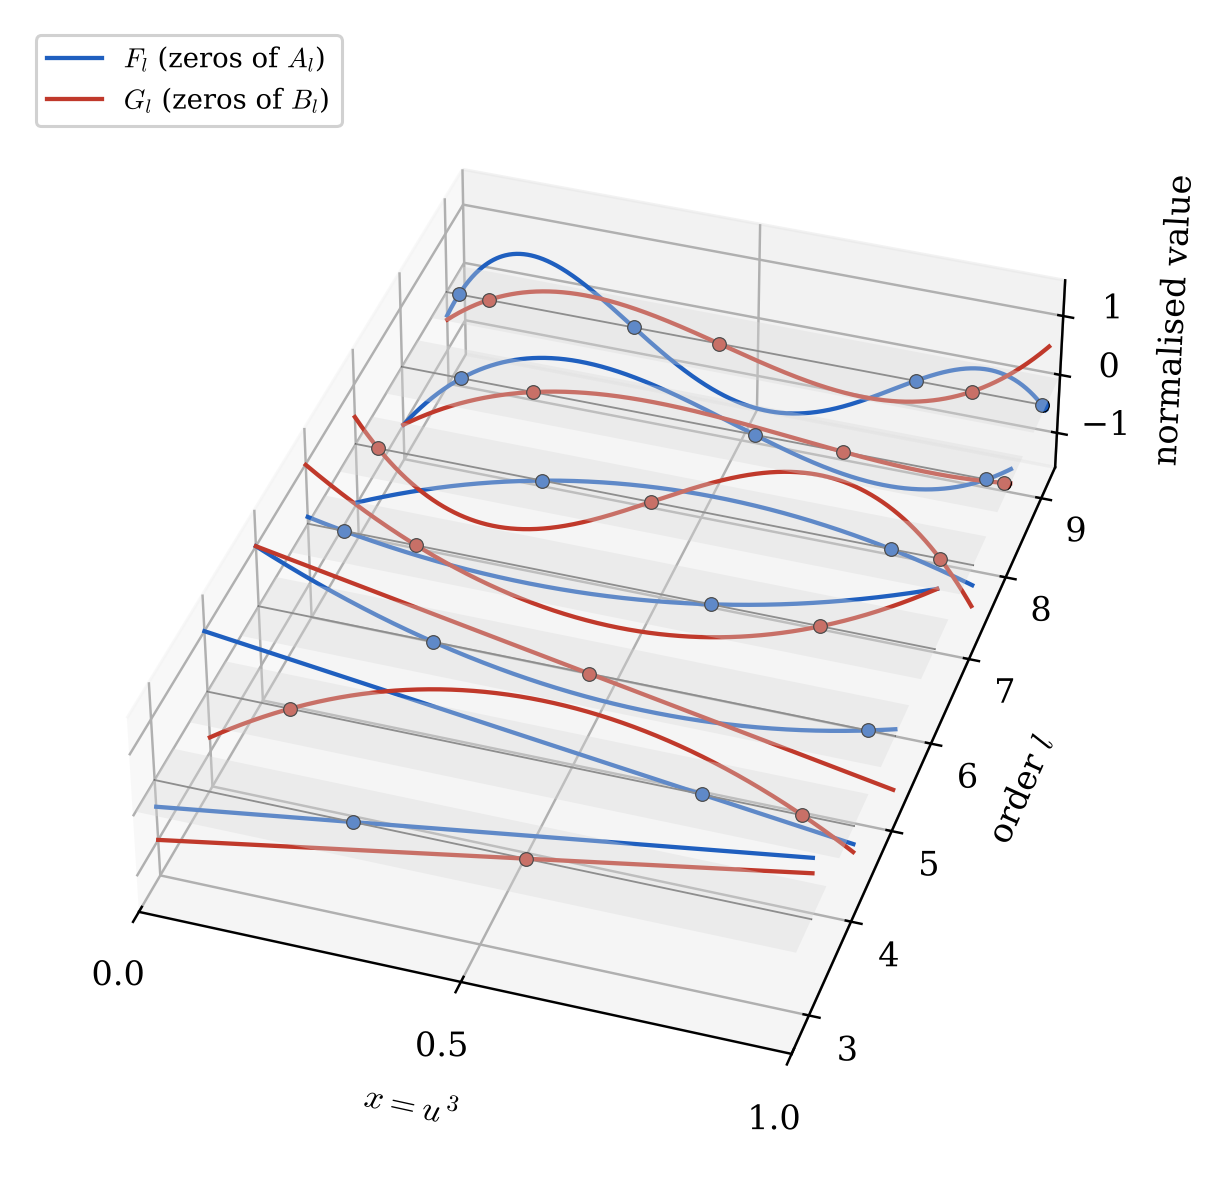
\includegraphics[width=0.9\textwidth]{fig_interlace.png}
\caption{The polynomials $F_l$ (blue) and $G_l$ (red) of \eqref{eq:phipsi} for $(p,q)=(2,3)$ and $l=3,\dots,9$, each scaled to maximum modulus one on $[0,1]$ and plotted against $x=u^3$. Their zeros, marked by dots, are those of $\varphi_l$ and $\psi_l$ in $(0,1)$, and they interlace at every order (Theorem~\ref{thm:interlace}).}
\label{fig:interlace}
\end{figure}

\begin{proof}[Proof of Theorem~\ref{thm:gcd}]
Let $(a_0,b_0)\in\C^2$ be a common zero of $A_l$ and $B_l$ with $a_0b_0\ne0$. By Lemma~\ref{lem:transport}, $(u_0,v_0)=(b_0/\mu,a_0/\kappa)$ is a common zero of $\Phi_l$ and $\Psi_l$ with $u_0v_0\ne0$, so $[u_0^N:v_0^M]$ is a common zero of $\tilde\Pi^A_l$ and $\tilde\Pi^B_l$. By Corollary~\ref{cor:forms} it equals $[x_0:1-x_0]$ with $x_0\in(0,1)$ and $F_l(x_0)=G_l(x_0)=0$, so $x_0$ is a common zero of $\varphi_l$ and $\psi_l$, contrary to Theorem~\ref{thm:interlace}. Hence every common zero lies on the axes. The greatest common divisor is weighted homogeneous, and an irreducible factor other than $a$ and $b$ would vanish at a point off the axes. So $\gcd(A_l,B_l)=a^{\min(\sigma_l,\sigma'_l)}b^{\min(\rho_l,\rho'_l)}$ by Lemma~\ref{lem:extreme}. With $r=(l-1)\bmod N$ we have $\rho_l=p-r$ and $\rho'_l=(p+1-r)\ind{r\ge1}$, so the minimum is $(p-r)\ind{r\ge1}$; likewise $\min(\sigma_l,\sigma'_l)=(q-s)\ind{s\ge1}$.
\end{proof}

\section{A weighted B\'ezout count}\label{sec:bezout}

From now on $p,q\ge2$. Fix $m\ge0$, put $l=m+1$, and let $F=A_l+U$, $G=B_l+V$ with $(U,V)\in\Omega$ as in Lemma~\ref{lem:degcount}. By \eqref{eq:deltabig}, every element of $V_m$ has weighted components of weight less than $W_A(l)$ and less than $W_B(l)$: indeed $W_A(j)\le W_A(l)-\delta$, $W_B(j)\le W_B(l)-\delta$ and $|W_A(j)-W_B(j)|=|\alpha-\beta|<\delta$ for $j\le m$. Let $S=K[Z,a,b]$, graded by $\wt Z=1$, $\wt a=\alpha$, $\wt b=\beta$, and let $F^h,G^h\in S$ be the weighted homogenisations of $F,G$ to weights $W_A=W_A(l)$ and $W_B=W_B(l)$. Then $F^h|_{Z=0}=A_l$ and $G^h|_{Z=0}=B_l$.

For $\lambda\in\{a,b\}$ write $\ell_\lambda$ for the intersection multiplicity at the origin of the curves obtained from $F^h$ and $G^h$ by setting $\lambda=1$, namely
\[
\ell_a=\dim_K K[Z,b]_{(Z,b)}\big/\bigl(F^h(Z,1,b),G^h(Z,1,b)\bigr),
\]
and $\ell_b$ the same with $a$ and $b$ exchanged.

\begin{proposition}\label{prop:bezout}
For $(U,V)$ in a dense open subset of $\Omega$,
\[
\deg X_m=\frac{W_AW_B}{\alpha\beta}-\frac{\ell_a}{\alpha}-\frac{\ell_b}{\beta}.
\]
\end{proposition}

\begin{proof}
\emph{Regular sequence.} A common factor $H$ of $F^h$ and $G^h$ of positive weight is weighted homogeneous and not divisible by $Z$, because $Z$ divides neither $F^h$ nor $G^h$. Then $H(1,a,b)$ is a nonconstant common factor of $F$ and $G$, which is impossible because $F$ and $G$ have finitely many common zeros. Hence $F^h,G^h$ is a regular sequence in $S$ and $M_\bullet=S/(F^h,G^h)$ is a graded Cohen--Macaulay module of dimension one, with Hilbert series
\[
\sum_{d\ge0}\dim_K M_d\,t^d=\frac{(1-t^{W_A})(1-t^{W_B})}{(1-t)(1-t^\alpha)(1-t^\beta)}
\]
\cite[Chapter~4]{BH98}. Its Hilbert function is eventually periodic, and its average, $\lim_{t\to1^-}(1-t)\sum_d\dim M_dt^d$, equals $W_AW_B/(\alpha\beta)$.

\emph{Decomposition.} Let $T\subset M_\bullet$ be the submodule annihilated by a power of $Z$ and $M'=M_\bullet/T$. The associated primes of $M'$ do not contain $Z$; they are the ideals $P_x=(a-x_1Z^\alpha,\,b-x_2Z^\beta)$ of the common zeros $(x_1,x_2)\in K^2$ of $F$ and $G$, and $S/P_x\cong K[Z]$. A graded composition series of $M'$ has factors $S/Q$ with $Q\supseteq P_x$ for some $x$, each finite over $K[Z]$. Hence $M'$ is a finitely generated torsion-free graded $K[Z]$-module, so it is free, and its rank is $\dim_K M'[Z^{-1}]_0=\dim_K M_\bullet[Z^{-1}]_0=\dim_KK[a,b]/(F,G)=\deg X_m$ by Lemma~\ref{lem:degcount}. The Hilbert function of $M'$ is eventually equal to $\deg X_m$.

\emph{The torsion.} $T$ is supported on $V(Z,A_l,B_l)$, which by Theorem~\ref{thm:gcd} consists of the irrelevant ideal and at most the two lines $P_a=(Z,b)$ and $P_b=(Z,a)$. A graded composition series of $T$ has factors isomorphic to shifts of $S/P_a\cong K[a]$, of $S/P_b\cong K[b]$ and of $K$; the number of factors $S/P_\lambda$ is $\length(T_{P_\lambda})=\length(M_{P_\lambda})$, since no $P_x$ is contained in $P_\lambda$. The Hilbert function of a shift of $K[a]$ is eventually periodic with average $1/\alpha$, and that of $K[b]$ with average $1/\beta$. Averaging the Hilbert function of $0\to T\to M_\bullet\to M'\to0$ gives
\[
\frac{W_AW_B}{\alpha\beta}=\frac{\length M_{P_a}}{\alpha}+\frac{\length M_{P_b}}{\beta}+\deg X_m .
\]

\emph{The lengths.} Let $\mathfrak m=(Z,b,a-1)$. The only minimal prime of the one-dimensional Cohen--Macaulay module $M_{\mathfrak m}$ is $P_a$, and $a-1$ is a parameter for it. By the associativity formula for multiplicities \cite[Chapter~4]{BH98},
\[
\length\bigl(M_{\mathfrak m}/(a-1)M_{\mathfrak m}\bigr)=e\bigl(a-1;M_{\mathfrak m}\bigr)=\length(M_{P_a})\cdot e\bigl(a-1;K[a]_{(a-1)}\bigr)=\length(M_{P_a}).
\]
The left side is $\ell_a$, since $M/(a-1)M=K[Z,b]/(F^h(Z,1,b),G^h(Z,1,b))$. In the same way $\length M_{P_b}=\ell_b$.
\end{proof}

\section{The two points at infinity}\label{sec:local}

We keep the notation of Section~\ref{sec:bezout}, with $l=m+1$, and compute $\ell_a$. Let $\lambda=l\bmod N$, so that $r=m\bmod N=(\lambda-1)\bmod N$.

\begin{proposition}\label{prop:local}
For $(U,V)$ in a dense open subset of $\Omega$,
\[
\ell_a=(p-r)\,r\,\delta,\qquad \ell_b=(q-s)\,s\,\delta .
\]
\end{proposition}

\begin{proof}
Put $f(Z,b)=F^h(Z,1,b)$ and $g(Z,b)=G^h(Z,1,b)$. Each term of $f$ is $Z^e$ times a term $b^j$ of $A_l(1,b)$ ($e=0$), of $A_{l-t}(1,b)$ ($e=t\delta$), of $B_{l-t}(1,b)$ ($e=\alpha-\beta+t\delta$), or of $1$ ($e=W_A$), with $1\le t\le l$, and the coefficient of $A_{l-t}$ and $B_{l-t}$ in $U$ multiplies it. The same holds for $g$ with $e=\beta-\alpha+t\delta$ for $A_{l-t}$, $e=t\delta$ for $B_{l-t}$ and $e=W_B$ for $1$. By Lemma~\ref{lem:extreme}, the $b$-exponents $j$ of $A_{l-t}$ satisfy $j\equiv t-\lambda$ and those of $B_{l-t}$ satisfy $j\equiv t+1-\lambda\pmod N$.

If $\lambda=0$, then $\rho_l=0$ and $A_l(1,0)\ne0$, so $f(0,0)\ne0$ and $\ell_a=0$; if $\lambda=1$, then $\rho'_l=0$ and $g(0,0)\ne0$. In both cases $r(p-r)=0$. Let now $2\le\lambda\le p$, so $r=\lambda-1\in[1,p-1]$, and put
\[
f_P=p+1-\lambda,\quad e_P=\alpha-\beta+(\lambda-1)\delta,\qquad f_Q=p+2-\lambda,\quad e_Q=(\lambda-1)\delta .
\]
These are positive by \eqref{eq:deltabig}. We claim that every term $Z^eb^j$ of $f$ satisfies $j/f_P+e/e_P\ge1$, that $f(0,b)$ has order exactly $f_P$, and that $f(Z,0)$ has order exactly $e_P$; and similarly for $g$ with $(f_Q,e_Q)$.

Indeed, $f(0,b)=A_l(1,b)$ has order $\rho_l=p+1-\lambda=f_P$ by Lemma~\ref{lem:extreme}. For a term coming from $A_{l-t}$: if $t\ge\lambda$ then $e=t\delta>e_P$; if $t<\lambda$ then $j\ge t-\lambda+N=f_P+t$, and $j e_P+e f_P\ge(f_P+t)e_P+t\delta f_P>f_Pe_P$. For a term coming from $B_{l-t}$: if $t\ge\lambda-1$ then $e\ge e_P$; if $t<\lambda-1$ then $j\ge t+1-\lambda+N=f_P+t+1$, and
\[
je_P+ef_P-f_Pe_P\ge(t+1)e_P+f_P(\alpha-\beta+t\delta)>0 .
\]
The constant term has $e=W_A>e_P$. Equality $j/f_P+e/e_P=1$ with $j=0$ occurs only for $B_{l-\lambda+1}$, whose index lies in $[1,m]$ and whose term free of $b$ exists by Lemma~\ref{lem:extreme}, because $1-(l-\lambda+1)\equiv0\pmod N$; no term from an $A_{l-t}$ has $e=e_P$ and $j=0$, since $j\equiv-1\pmod N$ when $t\delta=e_P$. Its coefficient in $U$ is free, so for generic $U$ the order of $f(Z,0)$ is $e_P$. The same computation for $g$ uses $g(0,b)=B_l(1,b)$ of order $\rho'_l=f_Q$. For $B_{l-t}$ with $t<\lambda-1$ we have $e=t\delta$ and $j\ge f_Q+t$, so $je_Q+ef_Q-f_Qe_Q\ge te_Q+t\delta f_Q>0$; for $A_{l-t}$ with $t<\lambda$ we have $e=\beta-\alpha+t\delta$, $j\ge f_Q+t-1$ and
\[
je_Q+ef_Q-f_Qe_Q\ge f_Q(\beta-\alpha+t\delta)+(t-1)(\lambda-1)\delta>0;
\]
the remaining terms have $e\ge e_Q$. The term $Z^{e_Q}$ comes from $B_{l-\lambda+1}$ with a free coefficient in $V$, and as before no term from an $A_{l-t}$ has $e=e_Q$ and $j=0$.

So the Newton polygon of $f$ at the origin is the single segment from $(0,f_P)$ to $(e_P,0)$, and that of $g$ is the segment from $(0,f_Q)$ to $(e_Q,0)$, in the $(e,j)$-plane (Figure~\ref{fig:newton}). By the Weierstrass preparation theorem, $f$ is a unit times a Weierstrass polynomial of degree $f_P$ in $b$, and by the Newton--Puiseux theorem its roots $b_1(Z),\dots,b_{f_P}(Z)$ are Puiseux series of order $\sigma=e_P/f_P$. The intersection multiplicity is $\ell_a=\sum_i\ord_Zg(Z,b_i(Z))$ \cite[Sections~1.2 and~2.6]{CA00}. Now
\[
f_Pe_Q<f_Qe_P,
\]
because $f_Qe_P-f_Pe_Q=(\lambda-1)\delta+(p+2-\lambda)(\alpha-\beta)$, which is positive if $\alpha\ge\beta$, and if $\alpha<\beta$ it is at least $(\lambda-1)\delta-p(\beta-\alpha)$ with $\lambda\ge2$, and $\delta-p(\beta-\alpha)=(pq-1-pq+p^2)/g>0$. Hence $\sigma>e_Q/f_Q$. Every term $Z^eb^j$ of $g$ contributes order $e+j\sigma\ge e+je_Q/f_Q\ge e_Q$ along each $b_i$, with equality only for the term $Z^{e_Q}$; so $\ord_Zg(Z,b_i(Z))=e_Q$ and $\ell_a=f_Pe_Q=(p+1-\lambda)(\lambda-1)\delta=(p-r)r\delta$.

The derivation $D$, and with it the whole construction, is unchanged when $(a,p,A_l)$ and $(b,q,B_l)$ are exchanged, and this exchange swaps $F$ and $G$. Hence $\ell_b=(q-s)s\delta$. The finitely many genericity conditions used are open and nonempty.
\end{proof}

\begin{figure}[ht]
\centering
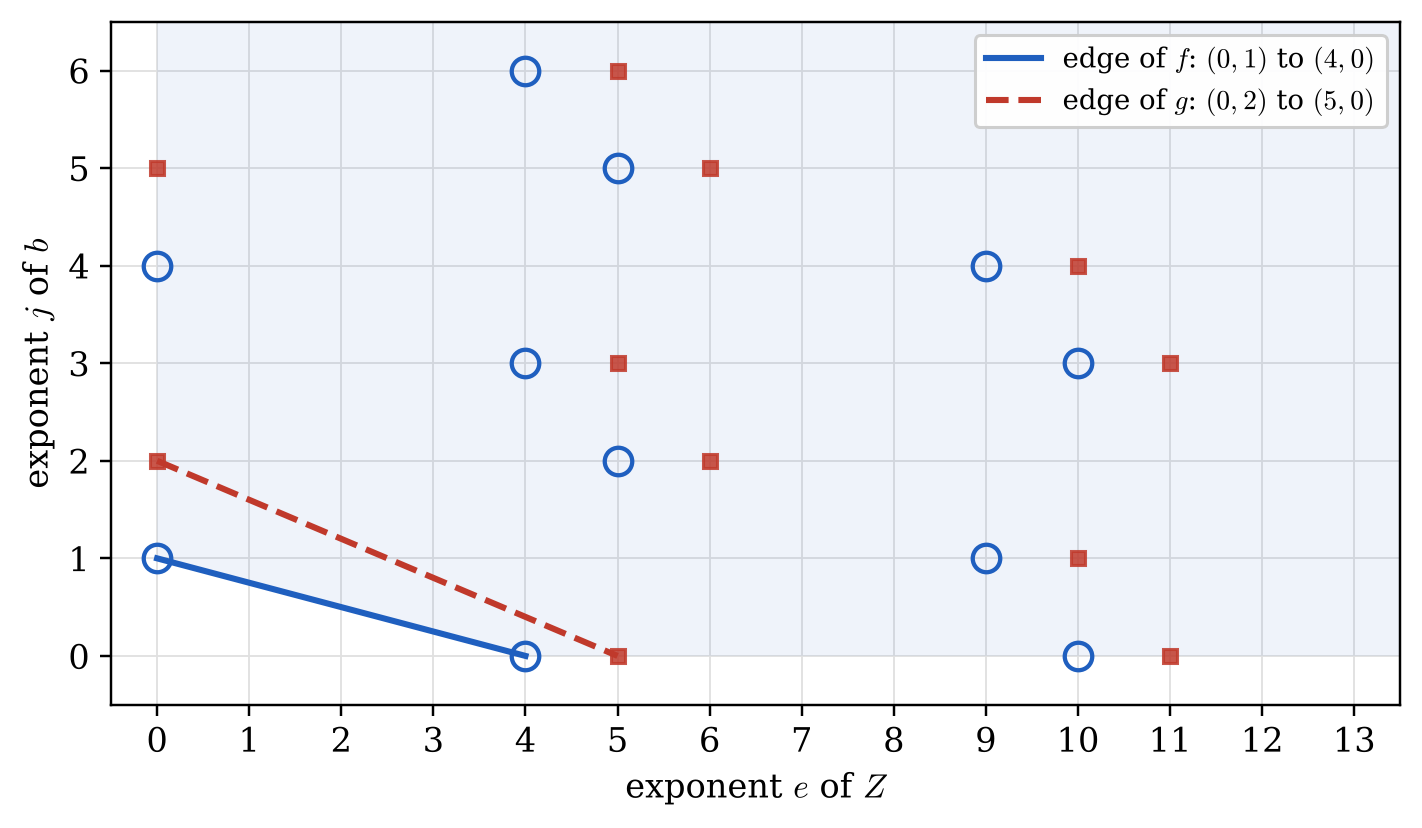
\includegraphics[width=0.78\textwidth]{fig_newton.png}
\caption{Terms $Z^eb^j$ of $f$ (circles) and $g$ (squares) at the point $[0:1:0]$ for $(p,q)=(2,3)$ and $m=4$, so that $\lambda=2$, $r=1$ and $\delta=5$. All terms lie on or above the edges from $(0,f_P)=(0,1)$ to $(e_P,0)=(4,0)$ and from $(0,f_Q)=(0,2)$ to $(e_Q,0)=(5,0)$, and the intersection multiplicity is $f_Pe_Q=5$.}
\label{fig:newton}
\end{figure}

\section{Proofs of the main results}\label{sec:proof}

\begin{proof}[Proof of Theorem~\ref{thm:main}]
By Propositions~\ref{prop:bezout} and~\ref{prop:local},
\[
\deg X_m=\frac{(\alpha+l\delta)(\beta+l\delta)}{\alpha\beta}-\frac{(p-r)r\delta}{\alpha}-\frac{(q-s)s\delta}{\beta},\qquad l=m+1 .
\]
Multiplying numerators and denominators by $g$ and using $g\alpha=p+1$, $g\beta=q+1$, $g\delta=c$, we get $g(\alpha+l\delta)=p+1+(m+1)c=p(q+1)+mc$ and $g(\beta+l\delta)=q(p+1)+mc$, which is the formula.
\end{proof}

\begin{proof}[Proof of Corollary~\ref{cor:pogudin}]
For $p=q=n$, $c=n^2-1$, the first term is $(n(n+1)+m(n^2-1))^2/(n+1)^2=((n-1)m+n)^2$, and the bracket is $2(n-1)r(n-r)$ because $s=r$. For $n=2$ this is $(m+2)^2-2\ind{r=1}$, and for $n=3$ it is $(2m+3)^2-4r(3-r)$, which is $(2m+3)^2-8$ for $r\in\{1,2\}$; this is \eqref{eq:pogudin}. For $(p,q)=(2,3)$, $c=5$ and the formula becomes the one in (ii); evaluating it gives the listed values. Part (iii) follows from the shape of the formula, since $r(p-r)/(p+1)$ depends only on $m\bmod(p+1)$ and $s(q-s)/(q+1)$ only on $m\bmod(q+1)$.
\end{proof}

\begin{remark}
Theorem~\ref{thm:gcd} and Section~\ref{sec:interlacing} hold for $p,q\ge1$, while \eqref{eq:deltabig} fails for $p=1$: then $\alpha-\beta=-\delta$, the jet $B_m$ has the same weight as $A_{m+1}$, and the highest weighted component of $A_{m+1}+U$ is $A_{m+1}+uB_m$ with a free coefficient $u$. The points at infinity are then the common zeros of $A_{m+1}+uB_m$ and $B_{m+1}$, and the method above needs an interlacing statement for this pencil. The degrees recomputed for the archive \cite{Archive} agree with the formula of Theorem~\ref{thm:main} also for $(p,q)=(1,2),(1,3),(1,5)$ and $m\le30$.
\end{remark}

\begin{remark}
The proof gives more than the degree. For generic $(U,V)$ the curves $A_{m+1}+U=0$ and $B_{m+1}+V=0$ in the weighted projective plane $\mathbb P(1,\alpha,\beta)$ \cite{Dol82} meet at infinity only at $[0:1:0]$ and $[0:0:1]$, with local ideals of the explicit lengths of Proposition~\ref{prop:local}, and all their affine intersection points are simple. Since $\mu^N/\kappa^M=-N/M$, Corollary~\ref{cor:forms} also shows that the zeros $z\ne0$ of $A_l(1,z)$ are exactly the solutions of $z^{p+1}=\frac{p+1}{q+1}\cdot\frac{x}{x-1}$ with $x$ a zero of $F_l$; in particular every such $z^{p+1}$ is a negative real number.
\end{remark}

\section*{Declarations}

\subsection*{Data availability}
No data were generated or analysed. Scripts that recompute the degrees of $X_m$ for thirteen pairs $(p,q)$ and $m\le30$, compare them with Theorem~\ref{thm:main} and test Theorem~\ref{thm:gcd} for small $p,q,l$ are archived with the source of this paper on Zenodo, version 1.0.0, \doi{10.5281/zenodo.24094790} \cite{Archive}; no proof in the paper depends on them.

\subsection*{Funding}
No funding was received for conducting this study.

\subsection*{Conflict of interest}
The author has no conflicts of interest to declare that are relevant to the content of this article.

\begingroup\raggedright
\begin{thebibliography}{99}

\bibitem{BhaBSD} D.~Bhattacharjee, \emph{The $p$-primary part of the Tate--Shafarevich group in ranks three to six: paper, data and certificates}, version 1.0.2, Zenodo, 2026. \doi{10.5281/zenodo.23933270}

\bibitem{BhaLehmer} D.~Bhattacharjee, \emph{A sixteen-prime-factor bound for Lehmer's totient problem and exact prime-completion criteria}, version 1.11.0, Zenodo, 2026. \doi{10.5281/zenodo.23795673}

\bibitem{BhaClass} D.~Bhattacharjee, \emph{Split primes and the exponent of imaginary quadratic class groups: paper, certification script and data}, version 1.0.0, Zenodo, 2026. \doi{10.5281/zenodo.24093928}

\bibitem{BH98} W.~Bruns and J.~Herzog, \emph{Cohen--Macaulay Rings}, revised ed., Cambridge Studies in Advanced Mathematics \textbf{39}, Cambridge University Press, Cambridge, 1998. \doi{10.1017/CBO9780511608681}

\bibitem{CA00} E.~Casas-Alvero, \emph{Singularities of Plane Curves}, London Mathematical Society Lecture Note Series \textbf{276}, Cambridge University Press, Cambridge, 2000. \doi{10.1017/CBO9780511569326}

\bibitem{Dol82} I.~Dolgachev, \emph{Weighted projective varieties}, in: Group Actions and Vector Fields, Lecture Notes in Mathematics \textbf{956}, Springer, Berlin, 1982, 34--71. \doi{10.1007/BFb0101508}

\bibitem{EGL12} D.~E.~Edmunds, P.~Gurka and J.~Lang, \emph{Properties of generalized trigonometric functions}, J. Approx. Theory \textbf{164} (2012), 47--56. \doi{10.1016/j.jat.2011.09.004}

\bibitem{Fisk} S.~Fisk, \emph{Polynomials, roots, and interlacing}, preprint, 2006. \href{https://arxiv.org/abs/math/0612833}{arXiv:math/0612833}

\bibitem{Har92} J.~Harris, \emph{Algebraic Geometry: A First Course}, Graduate Texts in Mathematics \textbf{133}, Springer, New York, 1992. \doi{10.1007/978-1-4757-2189-8}

\bibitem{Lan26} L.~Lanciano, \emph{Degrees and directional defects of embedded algebraic vector bundles}, preprint, 2026. \href{https://arxiv.org/abs/2609.27047}{arXiv:2609.27047}

\bibitem{Pog25} G.~Pogudin, \emph{Some open problems in differential algebra}, 24 January 2025. \url{https://www.lix.polytechnique.fr/Labo/Gleb.POGUDIN/files/da_problems.pdf}

\bibitem{Pud26} M.~Puddu, \emph{On the geometric degree of the prolongation varieties of the differential system $x_1'=x_2^2$, $x_2'=x_1^2$}, preprint, 2026. \href{https://arxiv.org/abs/2611.06638}{arXiv:2611.06638}

\bibitem{Ritt} J.~F.~Ritt, \emph{Differential Algebra}, American Mathematical Society Colloquium Publications \textbf{33}, American Mathematical Society, New York, 1950. \doi{10.1090/coll/033}

\bibitem{vL25} B.~S.~van Lith, \emph{Derivative polynomials and infinite series for squigonometric functions}, preprint, 2025. \href{https://arxiv.org/abs/2503.19624}{arXiv:2503.19624}

\bibitem{Archive} D.~Bhattacharjee, \emph{Degrees of Prolongation Varieties of Monomial Planar Systems}, version 1.0.0 (source, scripts and data), Zenodo, 2026. \doi{10.5281/zenodo.24094790}

\end{thebibliography}
\endgroup

\end{document}
